%%%%%%%%%%%%%%%%%%%%%%%%%%%%%%%%%%%%%%%%%%%%%%%%%%%%%%%%%%%%%%%%%%%%%%%%%%%%%%%


% Source: https://tug.org/pracjourn/2008-1/mori/mori.pdf
%%%%%%%%%%%%%%%%%%%%%%%%%%%%%%%%%%%%%%%%%%%%%%%%%%%%%%%%%%%%%%%%%%%%%%%%%%%%%%%

%%%%%%%%%%%%%%%%%%%%%%%%%%%%%%%%%%%%%%%%%%%%%%%%%%%%%%%%%%%%%%%%%%%%%%%%%%%%%%%
% Set a class and packages
\documentclass[11pt,a4paper,oneside]{book}

\usepackage[utf8]{inputenc}
\usepackage[T1]{fontenc}
\usepackage[brazil]{babel}
\usepackage[width=150mm,top=40mm,bottom=30mm,headsep=10mm,headheight=5mm]{geometry}
\usepackage{graphicx}
\usepackage{amssymb}
\usepackage{amsmath}
\usepackage{hyperref}
% create fancy headers
\usepackage{fancyhdr}
% commands for managing dates and its formats
\usepackage{datetime2}
% improved urls with proper hyphenation
\usepackage{xurl}
% Import enumitem to customize descriptions in license.tex
\usepackage{enumitem}
% Make caption titles bold
\usepackage[labelfont=bf,font=small,skip=0pt]{caption}
% To control the style of section titles
\usepackage{titlesec}
% Add the bibliography to the table of contents
\usepackage[nottoc,chapter]{tocbibind}
\usepackage[round,authoryear,sort]{natbib}
% Use custom apalike bibliography style
\bibliographystyle{apalike-doi}
% show dois as links on references
\usepackage{doi}
% Icon fonts (requires using xelatex or luatex)
\usepackage[fixed]{fontawesome5}
\usepackage{academicons}
% Set fonts (requires compilation with xelatex)
\usepackage{fontspec}
%%%%%%%%%%%%%%%%%%%%%%%%%%%%%%%%%%%%%%%%%%%%%%%%%%%%%%%%%%%%%%%%%%%%%%%%%%%%%%%

%%%%%%%%%%%%%%%%%%%%%%%%%%%%%%%%%%%%%%%%%%%%%%%%%%%%%%%%%%%%%%%%%%%%%%%%%%%%%%%
% Configuration of the document

\setmainfont[%
  Path = fonts/notoserif/,
  UprightFont = NotoSerif-Regular,
  BoldFont = NotoSerif-Bold,
  ItalicFont = NotoSerif-Italic,
  Extension = .ttf
]{NotoSerif}

% Increase the line spacing
\renewcommand{\baselinestretch}{1.5}

% Customize how Chapter headings are displayed
\titleformat{\chapter}[display]{\normalfont\bfseries}{\vspace{-3cm}}{5pt}{\Huge}

% Variables
\newcommand{\Author}{%
  Leonardo Uieda
}
\newcommand{\Year}{%
  2022
}

% Configure hyperref and add PDF metadata
\hypersetup{
    colorlinks,
    allcolors=[rgb]{0, 0.451, 0.753},
    pdftitle={Memorial para concurso publico de Professor Doutor na USP},
    pdfauthor={\Author},
    pdftex,
}

% make urls use the same font as every other text
\urlstyle{same}

% Define emptypage command
\newcommand{\emptypage}{%
    \newpage
    \thispagestyle{empty}
    \mbox{}
    \newpage
}

% Configure headers and footers
%==============================================================================
% Configure every page with a fancy style
\pagestyle{fancy}

% Define a command for configuring headers and footers of frontmatter
\newcommand{\fancyfront}{%
    \fancyhf{} % clear all header and footer fields
    \fancyfoot[C]{\thepage}
    \renewcommand{\headrulewidth}{0pt}
    \renewcommand{\footrulewidth}{0pt}

    % Override headers and footers for chapter pages
    \fancypagestyle{plain}{%
        \fancyhf{} % clear all header and footer fields
        \fancyfoot[C]{\thepage}
        \renewcommand{\headrulewidth}{0pt}
        \renewcommand{\footrulewidth}{0pt}
    }
}

% Define a command for configuring headers and footers of mainmatter
\newcommand{\fancymain}{%
    \fancyhf{} % clear all header and footer fields
    \fancyhead[RO,LE]{\thepage}
    \fancyhead[RE]{\leftmark}
    \fancyhead[LO]{\nouppercase{\rightmark}}
    \renewcommand{\headrulewidth}{0.4pt}

    % Override headers and footers for chapter pages
    \fancypagestyle{plain}{%
        \fancyhf{} % clear all header and footer fields
        \renewcommand{\headrulewidth}{0pt}
        \renewcommand{\footrulewidth}{0pt}
    }

}

% Clear headers and footers on blank pages before new chapter
\makeatletter
\def\cleardoublepage{
    \clearpage
    \if@twoside
        \ifodd\c@page
        \else\hbox{}\thispagestyle{empty}\newpage
            \if@twocolumn\hbox{}\newpage
            \fi
        \fi
    \fi
}
\makeatother
%==============================================================================
%%%%%%%%%%%%%%%%%%%%%%%%%%%%%%%%%%%%%%%%%%%%%%%%%%%%%%%%%%%%%%%%%%%%%%%%%%%%%%%

%%%%%%%%%%%%%%%%%%%%%%%%%%%%%%%%%%%%%%%%%%%%%%%%%%%%%%%%%%%%%%%%%%%%%%%%%%%%%%%
\begin{document}

\frontmatter
\fancyfront

\begin{titlepage}
  \begin{center}
    
\includegraphics[height=2cm]{images/logo.pdf}
    \vspace{1cm}

    MEMORIAL PARA CONCURSO PÚBLICO

    PROFESSOR DOUTOR (RDIDP) EM MÉTODOS POTENCIAIS

    UNIVERSIDADE DE SÃO PAULO
    \vspace{4cm}

    \textbf{\LARGE \MakeUppercase{\Author{}}}
    \vspace{5cm}

    \begin{minipage}[t]{0.6\textwidth}
      \begin{center}
        {\small
          Apresentado para concurso público de títulos e provas para cargo de
          Professor Doutor junto ao Departamento de Geofísica do Instituto de
          Astronomia, Geofísica e Ciências Atmosféricas da Universidade de São
          Paulo.
          \\
          Edital ATAc-IAG/044/2022
        }
      \end{center}
    \end{minipage}
    \vfill

    \Year{}
  \end{center}
\end{titlepage}

% Indice
\tableofcontents

\mainmatter
\fancymain

%==============================================================================
\chapter{Introdução}

Tive meu primeiro contato com a ciência e o ensino superior observando o
trabalho dos meus pais, ambos professores do Instituto de Biociências da
Universidade Estadual Paulista ``Júlio de Mesquita Filho'' (UNESP) de Botucatu,
São Paulo.
Até hoje associo as bancadas de microscópios e o cheiro de formol com o
conceito de ciência, mesmo nunca tendo trabalho em um laboratório com essas
características.
A curiosidade, a dedicação e a ética dos meus pais formaram a base da minha
posição a respeito da ciência e do que significa ser um educador.

\begin{figure}[h]
  \vspace{0.5cm}
  \begin{center}
    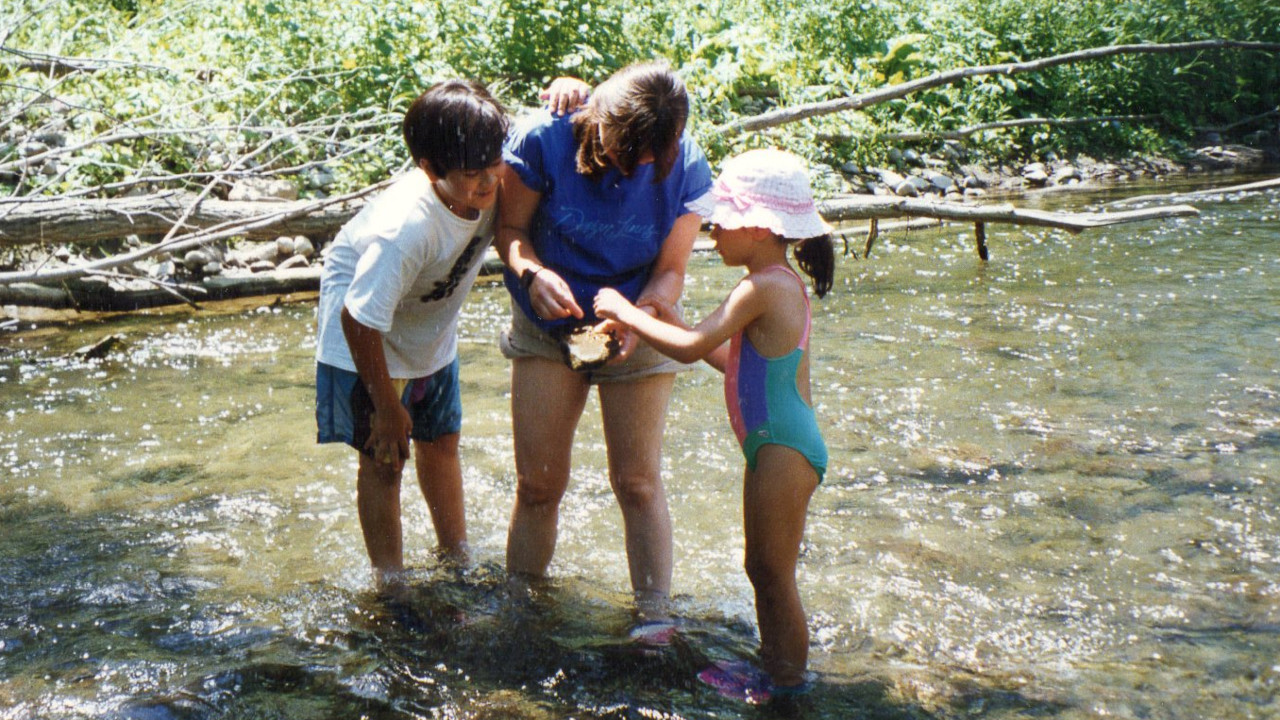
\includegraphics[width=\textwidth]{images/1997-06-ithaca-creek.jpg}
  \end{center}
  \caption{
    Bla
  }
  \label{fig:example}
\end{figure}


%==============================================================================
\chapter{Formação}

%==============================================================================
\chapter{Linhas de Pesquisa}

%==============================================================================
\chapter{Experiência em Ensino}

%==============================================================================
\backmatter
%\phantomsection  % use phantomsection to fix bibliography href in the toc
\bibliography{references}

\end{document}
